\begin{block}{synthesizing pdfs for decision relevance}
    If there are only a few PDFs, then qualitative comparisions (\eg, \cref{fig:tradeoffs}) may be sufficient.
    With \emph{many} PDFs (\eg, \cref{fig:boxplots}, refs.~\cite{ruckert_coastal:2019,sharma_rcp:2021}), further synthesis is needed.\\[0.5em]
    We consider the \emph{common case} of assessing decisions using simulations (SOWs) from each of $K$ PDFs.
    A system model $f$ quantifies the outcomes $u$ of taking decision $x$ under SOW $s$.
    Examining all SOWs created by a given model yields \emph{scenario-conditional optimization} (\cref{fig:tradeoffs}).
    To synthesize across PDFs, a weighting approach based on Bayesian Model Averaging \cite{wong_surge:2018,Yao:2018bu} is used.
    \begin{figure}
        \centering
        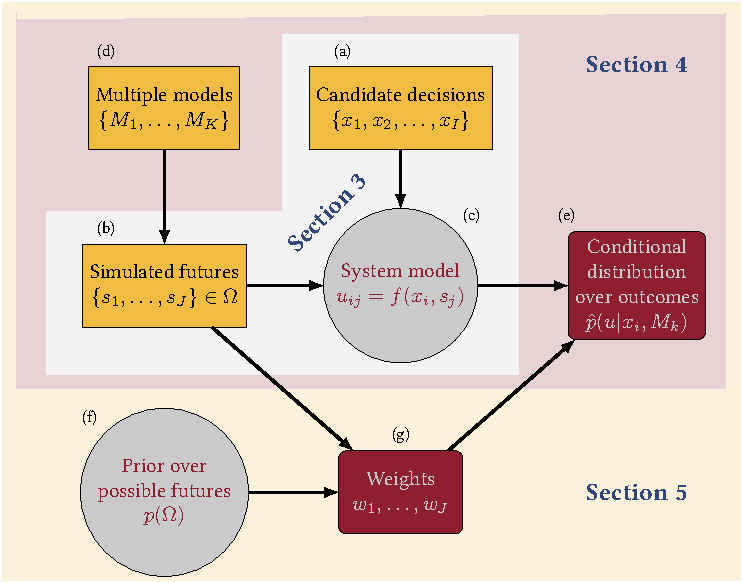
\includegraphics[width=0.9\textwidth]{bayes-rdm.pdf}
        \caption{
            Sketch of the ``Prior Model Averaging'' framework.
        }\label{fig:flowchart}
    \end{figure}
\end{block}